\documentclass[11pt,a4paper]{article}

\usepackage{fontspec}
\usepackage[a4paper,margin=2.5cm]{geometry}
\usepackage{booktabs}
\usepackage{longtable}
\usepackage{array}
\usepackage{graphicx}
\usepackage{subcaption}
\usepackage{xcolor}
\usepackage{amsmath,amssymb}
\usepackage{enumitem}
\usepackage{microtype}
\usepackage{caption}
\usepackage[numbers]{natbib}
\usepackage{parskip}
\usepackage{titlesec}
\usepackage[hidelinks]{hyperref}

\definecolor{linkviolet}{HTML}{6D28D9}
\hypersetup{
  colorlinks=true,
  linkcolor=linkviolet,
  citecolor=linkviolet,
  urlcolor=linkviolet,
  pdftitle={A multi-layer music recommender for Last.fm (HetRec2011)},
  pdfauthor={Sara Fibla Salgado}
}

\titleformat{\section}{\Large\bfseries}{\thesection}{0.6em}{}
\titleformat{\subsection}{\large\bfseries}{\thesubsection}{0.6em}{}

% Long unbreakable \code{} identifiers (snake_case function/file names)
% otherwise produce visible overfull lines in justified text; allow more
% inter-word stretch as a fallback before that happens.
\emergencystretch=3em
\tolerance=1200

\newcommand{\code}[1]{\texttt{#1}}
\newcommand{\secref}[1]{\S\ref{#1}}

\title{Recommender Systems: Individual Project Report\\[0.3em]
\Large A multi-layer music recommender for Last.fm (HetRec2011)}
\author{Sara Fibla Salgado\\[0.2em]\normalsize Recommender Systems, Prof.\ Marc Torrens}
\date{\today}

\begin{document}
\maketitle

\section{Introduction}
\label{sec:intro}

This project builds a recommender-system prototype for the music track of the assignment, using the Last.fm HetRec2011 dataset instead of MovieLens. The choice was deliberate: Last.fm ships three independent data layers (listening behaviour, folksonomy tags, and a social friend graph), where MovieLens only really offers one (ratings, plus a thin genre field). That gave room to do something the template's movie-domain skeleton doesn't: a social/friend-based recommender and a hybrid that fuses it with collaborative filtering, on top of the required baseline / content-based / CF / matrix-factorization set.

It also meant confronting a property MovieLens' explicit 1--5 star ratings hide: Last.fm's ``ratings'' are implicit feedback (raw play counts, no negative examples), which changes several algorithms' design from the ground up. Most importantly, matrix factorization is implemented as confidence-weighted ALS rather than SGD on a rating scale, for reasons explained in \secref{sec:als}.

\section{Dataset description}
\label{sec:dataset}

Source: GroupLens / HetRec 2011 workshop (5th ACM RecSys 2011), released for non-commercial research use. Retrieved via a public GitHub mirror of the original \code{hetrec2011-lastfm-2k.zip} archive (the canonical host, \code{files.grouplens.org}, was not reachable from this environment's network egress; the mirror's row counts were verified against the dataset's own published statistics before use).

\begin{table}[!htbp]
\centering
\begin{tabular}{lrl}
\toprule
File & Rows & Content \\
\midrule
\code{user\_artists.dat} & 92{,}834 & (user, artist, play count) \\
\code{artists.dat} & 17{,}632 & artist id, name, URL \\
\code{tags.dat} & 11{,}946 & tag vocabulary \\
\code{user\_taggedartists.dat} & 186{,}479 & (user, artist, tag) assignments \\
\code{user\_friends.dat} & 25{,}434 & directed friend edges (12{,}717 mutual) \\
\bottomrule
\end{tabular}
\caption{HetRec2011 Last.fm dataset files.}
\end{table}

1{,}892 users; 17{,}632 artists; matrix density 0.28\%.

\subsection{Why HetRec2011 over MSD Taste Profile or Spotify MPD}

All three were viable choices for the music track. MSD Taste Profile (user, song, play count triplets) and Spotify MPD (playlist-continuation) both recommend at song granularity, which HetRec2011 cannot: \code{user\_artists.dat} is the \emph{only} listening-interaction file in the dataset, and it is artist-level by construction. There is no track-level play data anywhere in HetRec2011 to recover, no matter how the pipeline is built. That is a real limitation of every recommendation in this project, baselines through hybrids, and is revisited in \secref{sec:discussion} and \secref{sec:prototype}. The trade-off that kept HetRec2011 the better fit here: MSD has no tags and no social graph, and Spotify MPD has neither either, plus it poses a fundamentally different problem (continue a playlist, not rank items for a user) that doesn't map onto the baseline/content-based/CF/matrix-factorization/social progression the assignment asks for. HetRec2011's three independent layers (\secref{sec:intro}) are what made the social-recommender and CF+social hybrid work possible at all; artist-level granularity was the cost of that, not an oversight.

\section{Preprocessing and EDA}
\label{sec:eda}

Key findings from \code{main.py}'s EDA step (see Figure~\ref{fig:eda}):

\begin{itemize}[leftmargin=*]
  \item Play counts are extremely heavy-tailed: mean 745, median 260, max 352{,}698. A handful of power-listeners would otherwise dominate every similarity computation, so every algorithm in this project works on $\log(1+\text{play count})$, not the raw count.
  \item Artist popularity follows a long tail: median listeners per artist is 1 (most artists in the catalog were listened to by exactly one person in this sample), while the top artists (Lady Gaga, Britney Spears, Rihanna, The Beatles, Katy Perry) have 470--611 listeners. This long tail is the direct cause of the collaborative-filtering bug described in \secref{sec:discussion}.
  \item The social graph is dense relative to the user base: every one of the 1{,}892 users has at least one friend, averaging 13.4 friends/user, enough for the friend-based recommender to have signal for essentially the whole population.
\end{itemize}

\begin{figure}[!htbp]
\centering
\begin{subfigure}{0.48\textwidth}
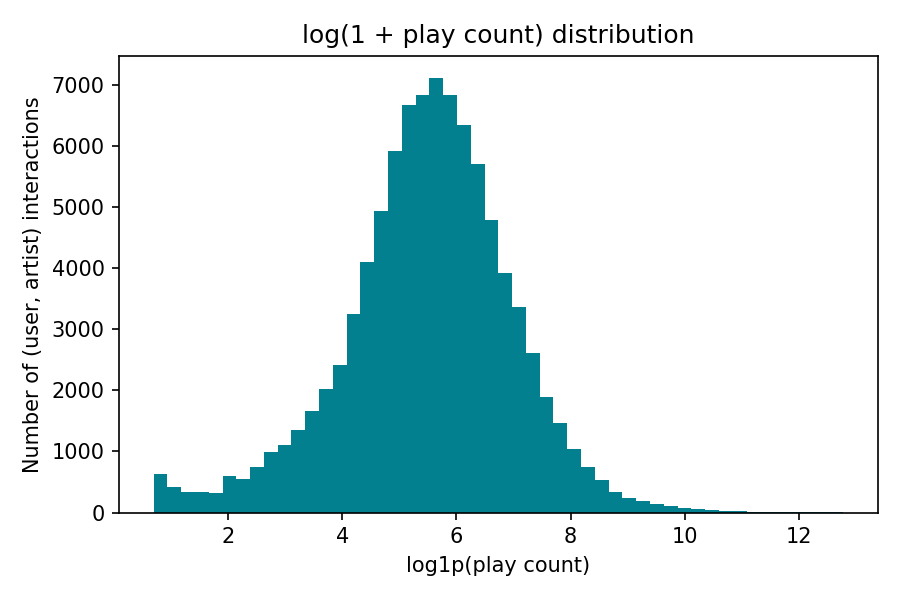
\includegraphics[width=\linewidth]{results/figures/play_count_distribution.png}
\caption{Play count distribution (heavy-tailed).}
\end{subfigure}
\hfill
\begin{subfigure}{0.48\textwidth}
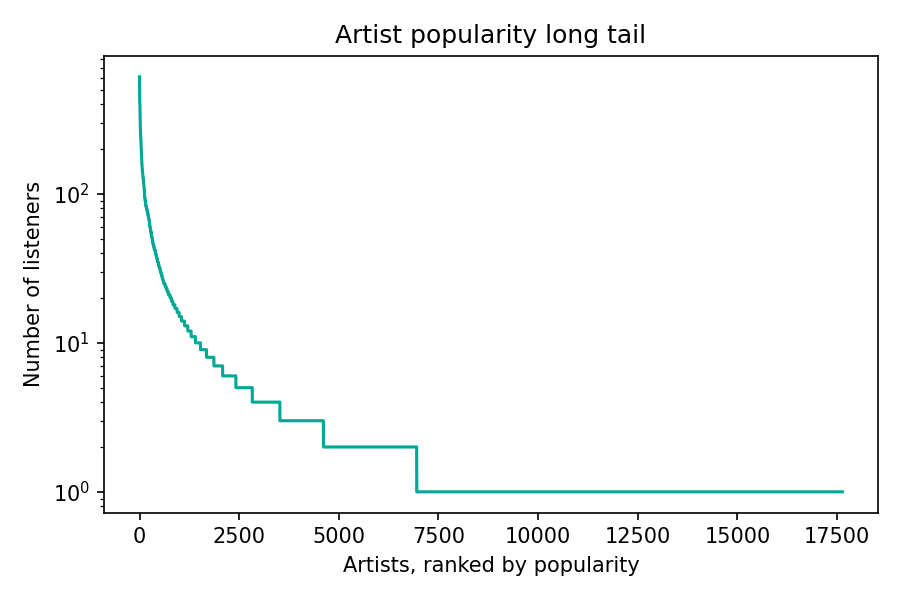
\includegraphics[width=\linewidth]{results/figures/popularity_long_tail.png}
\caption{Artist popularity long tail.}
\end{subfigure}
\par\bigskip
\begin{subfigure}{0.48\textwidth}
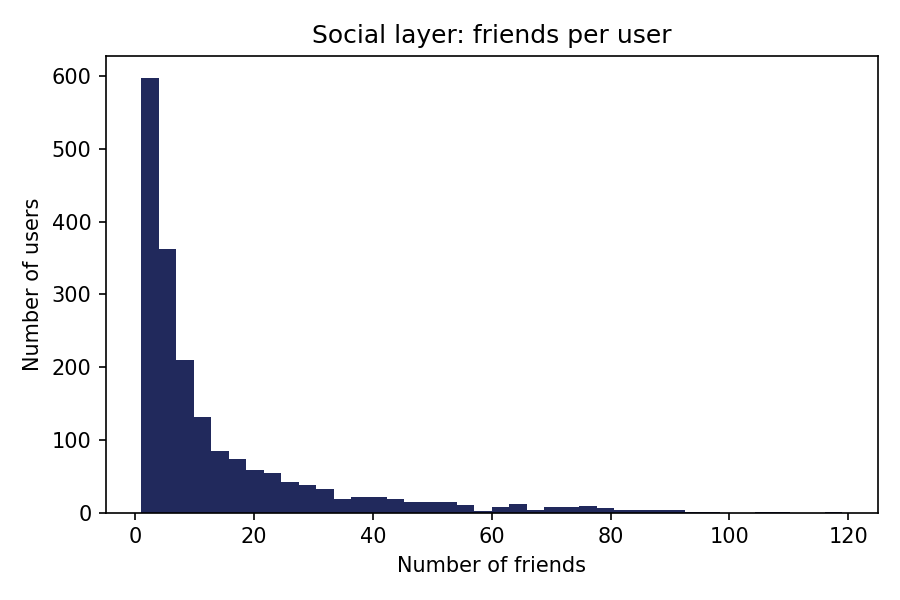
\includegraphics[width=\linewidth]{results/figures/friends_per_user.png}
\caption{Friends per user.}
\end{subfigure}
\hfill
\begin{subfigure}{0.48\textwidth}
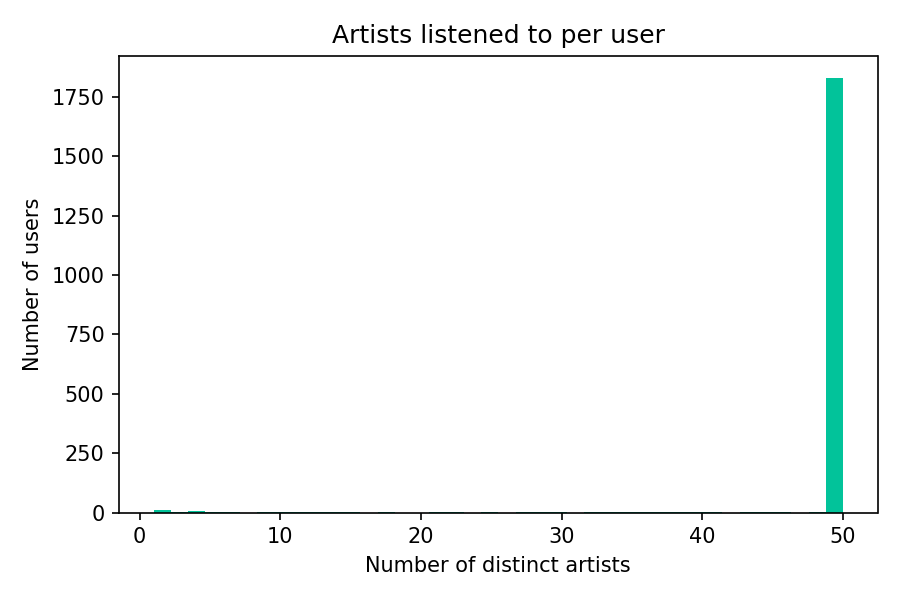
\includegraphics[width=\linewidth]{results/figures/interactions_per_user.png}
\caption{Interactions per user.}
\end{subfigure}
\caption{Exploratory data analysis of the HetRec2011 dataset.}
\label{fig:eda}
\end{figure}

\subsection{Train/test split}

Per-user random 80/20 split (not a single global split), so every evaluable user has both training history and held-out ground truth. Users with fewer than 5 interactions are kept entirely in training (not enough signal to hold out a meaningful test slice for them, but they still contribute to similarity/popularity estimation).

\subsection{Relevance for ranking metrics}

There is no 1--5 star scale to threshold on, so a held-out interaction counts as ``relevant'' if its play count is at or above \emph{that user's own median training play count}: one of the artists this user actually favoured, defined relative to their own behaviour rather than a fixed global cutoff.

\subsection{Encoding fix}

\code{artists.dat} is genuinely UTF-8, but an earlier version of the loader read it as \code{latin-1}. Both ``succeed'' (no decode error), but the latter silently mangles every accented name into mojibake (e.g.\ ``R\"oyksopp'' $\to$ ``Röyksopp''). Confirmed by checking which encoding actually round-trips: \code{tags.dat} \emph{fails} to decode as UTF-8 (it genuinely is latin-1, the 2011 export is inconsistent across files), while \code{artists.dat} decodes cleanly under both, so latin-1 was silently wrong there. This was cosmetic (doesn't touch any ID or similarity computation) but visible in every example output and the live app, so it's fixed in \code{data\_loading.load\_artists}.

\section{Algorithms implemented}
\label{sec:algorithms}

\subsection{Non-personalized baselines}

\begin{itemize}[leftmargin=*]
  \item Most Popular: ranked by number of unique listeners (not total plays, which would let one obsessive listener distort the ranking).
  \item Most Played: ranked by total play count, with a minimum-listener floor (the implicit-feedback analogue of ``highest average rating with a minimum number of ratings'').
  \item Random: sanity-check lower bound.
\end{itemize}

\subsection{Content-based (tags)}

TF-IDF over each artist's aggregated folksonomy tags (\code{user\_taggedartists.dat} joined with \code{tags.dat}). A user profile is the listening-weighted centroid of artists they've played:
\begin{equation}
\text{profile}(u) = \sum_i \big(\log\text{-}\text{play}(u,i) - \overline{\log\text{-}\text{play}}(u)\big) \cdot \text{vector}(i)
\end{equation}
centering by the user's own mean log-play-count, the implicit-feedback analogue of centering by mean rating. Recommendations are unseen artists with the highest cosine similarity to the profile.

\code{ContentBasedRecommender(use\_tfidf=...)} also supports raw tag-application counts (a plain \code{CountVectorizer}) instead of TF-IDF, specifically to run the comparison the assignment suggests as an extension. The result is counter-intuitive: raw counts beat TF-IDF on every accuracy metric (\secref{sec:results}); see the discussion there for why down-weighting ``common'' tags isn't automatically the right move on this dataset.

\subsection{Collaborative filtering (item-item and user-user)}

Cosine similarity over log-compressed play counts, deliberately not mean-centered the way the explicit-rating ``adjusted cosine'' would be (see the code docstrings for why centering is the wrong move for implicit, non-negative data). This is also where the most interesting debugging of the project happened; see \secref{sec:discussion}.

Neighbourhood size $k$ (how many top-similar neighbours contribute to a prediction) is tuned, not hand-picked, by the same inner-validation grid-search pattern as the hybrid weight (\secref{sec:protocol}). See \secref{sec:results} for what that search found: a genuine non-result, $k$ barely matters on this dataset.

\subsection{Matrix factorization: implicit ALS, not SGD}
\label{sec:als}

The explicit-rating model ($\hat{r} = \mu + b_u + b_i + p_u \cdot q_i$, trained with SGD on observed ratings) doesn't transfer to implicit data: there are no negative examples, so treating ``unobserved'' as ``rated zero'' would tell the model a user dislikes 99.7\% of the catalog, which isn't what missing data means here. Instead this project implements the standard implicit-feedback model \citep{hu2008collaborative}, trained with Alternating Least Squares:

\begin{align}
\text{preference} \quad & p_{ui} = 1 \text{ if the user played artist } i \text{ at all, else } 0 \\
\text{confidence} \quad & c_{ui} = 1 + \alpha \cdot \log(1 + \text{play\_count}_{ui}) \\
\text{model} \quad & \hat{p}_{ui} = x_u \cdot y_i
\end{align}

Every observed entry is a confidence-weighted positive; every unobserved entry still contributes (with confidence 1, preference 0). The model is explicitly told ``probably not interested'' for everything a user hasn't played, just much more lightly than for what they did play. Each update is an exact closed-form ridge-regression solve, not a noisy gradient step.

\begin{figure}[!htbp]
\centering
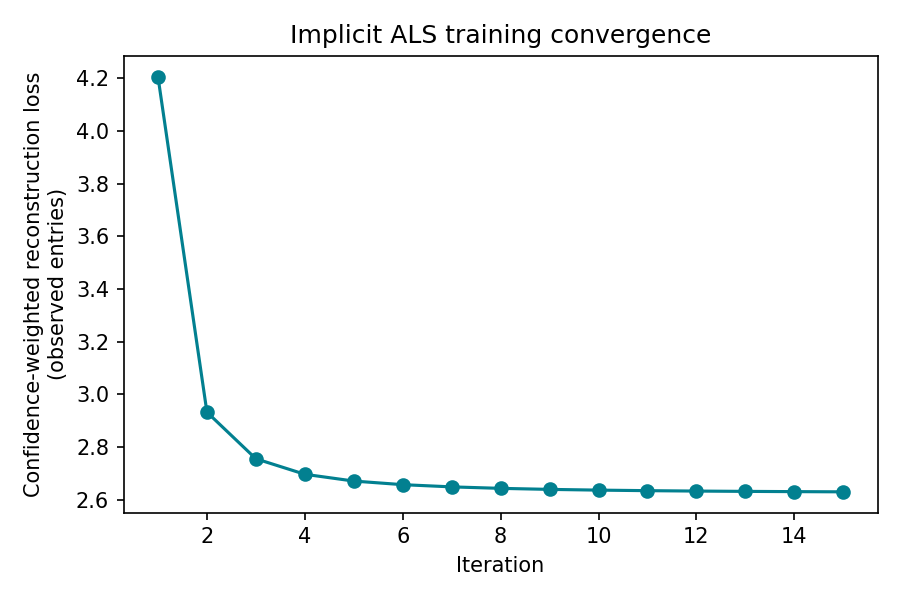
\includegraphics[width=0.65\linewidth]{results/figures/als_training_curve.png}
\caption{Implicit ALS training loss curve.}
\end{figure}

The number of latent factors, the regularization strength \code{reg}, and the confidence-scaling $\alpha$ shown above are all grid-searched on the same inner train/validation split as the hybrid weight and CF $k$ (\secref{sec:protocol}), rather than left at hand-picked defaults. See \secref{sec:results}: the validated factor count (20) turned out to \emph{beat} this project's original hand-picked default (50), which is itself evidence the original default was never actually checked. \code{reg}/$\alpha$ are tuned in a second pass, staged \emph{after} \code{n\_factors} rather than jointly (see \secref{sec:protocol}/\secref{sec:discussion} for why and what that trade-off cost), and the result was more mixed: a small, real win on some metrics and a small, real cost on others, not a clean improvement; see \secref{sec:results}.

\subsection{The social layer (the part a movie-only project couldn't have)}
\label{sec:social}

\subsubsection{Friend-Based}

Recommend artists popular among a user's actual Last.fm friends, weighted by each friend's own log-play-count.

\subsubsection{Graph Diffusion (Personalized PageRank)}

The same idea, extended past one hop. Friend-Based only ever looks at a user's \emph{direct} friends, so someone with one or two friends whose own listening is thin gets a correspondingly thin signal: the same local-neighbourhood limitation \secref{sec:discussion} diagnoses for item-item CF, and the reason Implicit ALS was brought in at all (latent-factor models borrow statistical strength across the \emph{whole} matrix instead of only directly-overlapping neighbours). \code{GraphDiffusionRecommender} (\code{src/social\_filtering.py}) applies the same fix to the social layer instead of the listening layer: Personalized PageRank \citep{page1999pagerank}, a random walk over the (symmetrized) friend graph that restarts at the query user with probability 0.15 at every step, computed by power iteration, gives every user in the network a continuous relevance weight to the query user, friends scoring highest and friends-of-friends progressively less, instead of a hard one-hop cutoff. See \secref{sec:results} for what extending the reach like this actually trades away.

\subsubsection{Hybrid (CF + Social)}

A generic weighted reciprocal-rank fusion of item-item CF and the friend-based recommender. Rank fusion (rather than blending raw scores) was used because every model here lives on a different, incomparable scale (cosine similarity vs.\ ALS dot product vs.\ summed log-play-counts), so converting each model's output to $1/(\text{rank}+1)$ before blending is the only way the combination means anything. The blend weight is no longer hand-picked: \code{tune\_hybrid\_weight()} grid-searches it on an inner train/validation split (carved out of the \emph{training} data only, never the test set; see \secref{sec:protocol}) and the production model uses whatever weight wins on held-out NDCG@10. See \secref{sec:discussion} for what that search actually found.

\subsubsection{Hybrid (ALS + Social)}

The same reciprocal-rank fusion, applied to this project's two most accurate \emph{individual} models, Implicit ALS and Graph Diffusion, rather than the strongest listening-layer model and the strongest social-layer model. \code{tune\_hybrid\_weight()}'s CF+Social search degenerated to a 100\% boundary weight (above); this is the natural follow-up question it raises: does blending the two strongest signals, regardless of which layer they come from, do any better than either alone? \code{tune\_als\_social\_hybrid\_weight()} answers it on the same inner train/validation split, by the same NDCG@10 selection rule. See \secref{sec:results}/\secref{sec:discussion} for what it found: a more interesting and more cautionary result than either of the other two hybrid searches in this project.

\subsection{Cold-start backfill}
\label{sec:backfill}

A real product never shows an empty results page. \code{BackfillRecommender} (\code{src/backfill.py}) wraps any fitted model and, if it returns fewer than $n$ items for a user (which happens for item-item/user-user CF when a user's neighbourhood never clears the minimum-support floor, or for the friend-based recommender when a user has no friends), tops up the list with Most-Popular picks until it reaches $n$. This is applied at the \emph{delivery} layer (the React/FastAPI prototype, \secref{sec:prototype}, backfills invisibly: no algorithm or fallback is ever surfaced to the user) rather than baked into the algorithms themselves, so the offline evaluation table in \secref{sec:results} still reports each algorithm's own, unmodified accuracy; \secref{sec:discussion} reports a separate before/after comparison quantifying the trade-off.

\subsection{Diversity-aware re-ranking (MMR)}
\label{sec:mmr}

\secref{sec:results} shows Implicit ALS is both the most accurate model in this project and one of the most popularity-biased, exactly the kind of measured-but-unmitigated weakness a re-ranking step exists to fix. \code{src/diversification.py} adds Maximal Marginal Relevance \citep{carbonell1998mmr} as a post-hoc re-ranking layer, the same wrapper pattern \code{BackfillRecommender} (\secref{sec:backfill}) already uses: it doesn't change how ALS is trained, it reorders ALS's own candidate pool to trade a controlled amount of relevance for less redundancy, scoring each remaining candidate $i$ against what's already been selected as

\begin{equation}
\text{MMR}(i) = \lambda \cdot \text{relevance}(i) - (1-\lambda) \cdot \max_{j \in \text{selected}} \text{sim}(i,j)
\end{equation}

using the same TF-IDF tag-cosine similarity \secref{sec:protocol} already uses to \emph{measure} diversity, so ``diversity'' means the same thing whether it's being measured or optimized for. $\lambda = 1$ is pure relevance (no diversification); lower $\lambda$ increasingly favours items dissimilar to what's already in the list.

\subsubsection{Picking \texorpdfstring{$\lambda$}{lambda}}

Maximizing validation NDCG would trivially always pick $\lambda = 1$ and defeat the point of the technique, so \code{tune\_mmr\_lambda()} instead sweeps $\lambda \in \{1.0, 0.9, \ldots, 0.1\}$ on the same inner train/validation split used elsewhere (\secref{sec:protocol}) and selects the most diversification (lowest $\lambda$) that keeps validation precision@10 within 10\% relative of the pure-relevance baseline: an explicit accuracy budget, not a blind metric maximization. The full sweep is a clean, monotonic Pareto curve (Figure~\ref{fig:mmr}, \code{results/mmr\_lambda\_sweep.csv}):

\begin{table}[!htbp]
\centering
\begin{tabular}{lrr}
\toprule
$\lambda$ & val P@10 & val diversity \\
\midrule
1.0 (baseline) & 0.0753 & 0.630 \\
0.8 & 0.0743 & 0.669 \\
0.6 (selected) & 0.0702 & 0.736 \\
0.4 & 0.0575 & 0.827 \\
0.1 & 0.0334 & 0.894 \\
\bottomrule
\end{tabular}
\caption{MMR $\lambda$ sweep on the inner validation split.}
\end{table}

$\lambda = 0.6$ is the lowest value with val P@10 still $\geq$ 90\% of baseline (0.0702 vs.\ a 0.0678 threshold), so that's what \code{matrix\_factorization\_mmr} uses in \secref{sec:results}'s evaluation table.

\section{Evaluation protocol}
\label{sec:protocol}

Precision@10, Recall@10, NDCG@10, MRR@10, Hit-Rate@10 (binary relevance per \secref{sec:eda}), plus four beyond-accuracy metrics, each answering a different question, and each required or suggested by the assignment:

\begin{itemize}[leftmargin=*]
  \item Catalog coverage: fraction of the entire training catalog that ever appears across all users' top-10 lists (``how much of the catalog gets recommended to \emph{anyone}''). A model that always recommends the same 10 superstar artists to everyone has near-zero coverage even if its precision looks fine.
  \item Novelty: mean self-information ($-\log_2 P(\text{artist})$, $P$ estimated from listener counts) of the recommended items (``how obscure is a typical recommendation''), the natural counterweight to popularity bias.
  \item Diversity: mean pairwise dissimilarity ($1 - $ cosine similarity of TF-IDF tag vectors) between the items \emph{within one user's list}. This is distinct from both: a model could have great coverage and novelty in aggregate while still giving any single user ten near-identical artists. Computed using the content-based recommender's tag vectors regardless of which algorithm produced the list, so every model is measured the same way.
  \item Popularity bias: mean popularity \emph{percentile} (0 = least popular item in the catalog, 1 = the single most popular item) of the recommended items. A fourth, deliberately different lens from the three above: coverage is about spread \emph{across users}, novelty is a log-scale absolute-popularity measure, and a model can score fine on both while still leaning on a handful of moderately-popular artists \emph{within} every individual list. Popularity bias catches that directly, on a scale that's easy to sanity-check (Random should land at $\approx 0.50$; it does, see \secref{sec:results}, which is a useful unit test for the metric itself).
\end{itemize}

\subsection{Parameter tuning}

Five hyperparameters/weights with no obviously correct default are grid-searched on an \emph{inner} 85/15 train/validation split carved out of the training data, rather than hand-picked (never the held-out test set, so nothing in \secref{sec:results} is contaminated by having been used to pick a hyperparameter):

\begin{itemize}[leftmargin=*]
  \item \code{tune\_model\_params()}: implicit-ALS latent factor count ($n_{\text{factors}} \in \{20, 50, 80\}$), then, staged \emph{after} $n_{\text{factors}}$ is fixed, not jointly, regularization $\text{reg} \in \{0.01, 0.05, 0.1, 0.3\}$ and confidence scaling $\alpha \in \{1.0, 2.0, 4.0, 8.0\}$ (16 combinations), and item-item-CF neighbourhood size ($k \in \{10, 20, 30, 50\}$), all selected by validation NDCG@10. The chosen $k$ is reused for user-user CF too, for simplicity. Staging \code{reg}/$\alpha$ after $n_{\text{factors}}$ rather than searching all three jointly keeps the grid small (16 fits instead of $3\times16=48$), at the cost of not exploring whether a different factor count would prefer different \code{reg}/$\alpha$; see \secref{sec:discussion} for whether that mattered.
  \item \code{tune\_hybrid\_weight()}: the CF/social blend weight (\secref{sec:social}), also by validation NDCG@10.
  \item \code{tune\_mmr\_lambda()}: the MMR relevance/diversity weight (\secref{sec:mmr}), the \emph{only} one of these not selected by maximizing validation NDCG, since that would trivially pick ``no diversification.'' Selected instead by an explicit accuracy-budget rule (most diversity subject to $\leq$10\% relative validation-precision loss); the full sweep, not just the selected point, is reported (\secref{sec:results}) because for a trade-off-by-design technique, the \emph{shape} of the trade-off is the actual evidence, not a single number.
  \item \code{tune\_als\_social\_hybrid\_weight()}: the Implicit ALS / Graph Diffusion blend weight (\secref{sec:social}), also by validation NDCG@10. See \secref{sec:results}/\secref{sec:discussion} for why this one's selected weight didn't hold up on the test set, unlike the other three.
\end{itemize}

\subsection{Statistical significance}

A bare comparison of two mean accuracy numbers in a table can't say whether a gap reflects a real, stable difference between two algorithms or noise from which 20\% of each user's history happened to land in the test set. \code{run\_significance\_tests()} runs a paired Wilcoxon signed-rank test (chosen over a paired t-test because per-user precision/NDCG@10 is bounded in $[0,1]$ and heavily zero-inflated, clearly not normally distributed) on per-user NDCG@10 for seven model pairs of interest, including Implicit ALS vs.\ its MMR-re-ranked variant (is the precision cost of diversification real, or noise?), Graph Diffusion vs.\ Friend-Based (\secref{sec:social}), and the ALS+Graph-Diffusion hybrid vs.\ plain ALS (is its validation-set win real on test, or not?). Results in \secref{sec:results}.

\subsection{Relevance-threshold robustness}

Every ranking metric in this report is defined relative to one specific, otherwise-unexamined choice: a held-out interaction counts as ``relevant'' if its play count is at or above the user's own \emph{median} training play count (\code{config.RELEVANCE\_PERCENTILE = 0.5}, \secref{sec:eda}). \code{relevance\_threshold\_check.py} re-evaluates a representative subset of models (one per paradigm) against two alternative definitions, ``any play counts'' ($q=0.00$) and a stricter ``favourite-tier only'' bar ($q=0.75$), fitting each model once on the standard split and only varying which held-out interactions count as a hit, so this is cheap to check without re-tuning or re-fitting anything. Results in \secref{sec:results}.

\subsection{Multi-seed robustness}

\code{robustness\_check.py} repeats the train/test split, model fitting, and evaluation across 5 random seeds (independent from the main pipeline, since it re-runs the most expensive step, fitting implicit ALS, once per seed) and reports mean $\pm$ std per model: a single train/test split's results could otherwise be mistaken for a stable property of the algorithm rather than one split's luck. See \secref{sec:results}.

\section{Results}
\label{sec:results}

\begin{table}[!htbp]
\centering
\scriptsize
\setlength{\tabcolsep}{4pt}
\begin{tabular}{lrrrrrrrrr}
\toprule
Model & P@10 & R@10 & NDCG@10 & MRR@10 & HR@10 & Cov. & Nov. & Div. & PopB. \\
\midrule
Most Popular & 0.0492 & 0.1010 & 0.0876 & 0.1516 & 0.319 & 0.002 & 2.43 & 0.638 & 1.000 \\
Most Played & 0.0433 & 0.0891 & 0.0747 & 0.1288 & 0.305 & 0.002 & 2.71 & 0.691 & 0.999 \\
Random & 0.0004 & 0.0006 & 0.0005 & 0.0010 & 0.004 & 0.700 & 10.01 & 0.990 & 0.501 \\
Content-Based (TF-IDF) & 0.0344 & 0.0708 & 0.0620 & 0.1182 & 0.266 & 0.278 & 8.39 & 0.316 & 0.662 \\
Content-Based (raw) & 0.0449 & 0.0917 & 0.0846 & 0.1611 & 0.323 & 0.209 & 7.33 & 0.321 & 0.767 \\
User-User CF & 0.0210 & 0.0437 & 0.0354 & 0.0672 & 0.183 & 0.149 & 6.67 & 0.854 & 0.878 \\
Item-Item CF ($k$=30) & 0.0141 & 0.0261 & 0.0229 & 0.0461 & 0.119 & 0.031 & 5.03 & 0.765 & 0.983 \\
Implicit ALS (tuned) & 0.1335 & 0.2756 & 0.2650 & 0.4383 & 0.695 & 0.039 & 4.05 & 0.637 & 0.992 \\
Implicit ALS + MMR ($\lambda$=0.6) & 0.1285 & 0.2664 & 0.2547 & 0.4343 & 0.683 & 0.038 & 4.07 & 0.742 & 0.992 \\
Friend-Based (social) & 0.0845 & 0.1735 & 0.1701 & 0.3007 & 0.486 & 0.165 & 4.83 & 0.701 & 0.945 \\
Graph Diffusion (PPR) & 0.0875 & 0.1796 & 0.1764 & 0.3094 & 0.496 & 0.095 & 3.97 & 0.644 & 0.975 \\
Hybrid (CF+social, 0/1) & 0.0846 & 0.1736 & 0.1702 & 0.3008 & 0.486 & 0.165 & 4.83 & 0.701 & 0.945 \\
Hybrid (ALS+GD, 0.8/0.2) & 0.1327 & 0.2748 & 0.2646 & 0.4392 & 0.694 & 0.045 & 3.92 & 0.657 & 0.991 \\
\bottomrule
\end{tabular}
\caption{Full model comparison @k=10.}
\label{tab:results}
\end{table}

(\code{results/metrics.csv} has the full precision table, \code{results/metrics\_backfilled.csv} has the cold-start-backfilled comparison, \code{results/significance\_tests.csv} has the Wilcoxon results, \code{results/metrics\_multiseed\_summary.csv} has the 5-seed mean/std, \code{results/mmr\_lambda\_sweep.csv} has the MMR $\lambda$ sweep, \code{results/relevance\_threshold\_check.csv} has the relevance-threshold robustness sweep.)

\begin{figure}[!htbp]
\centering
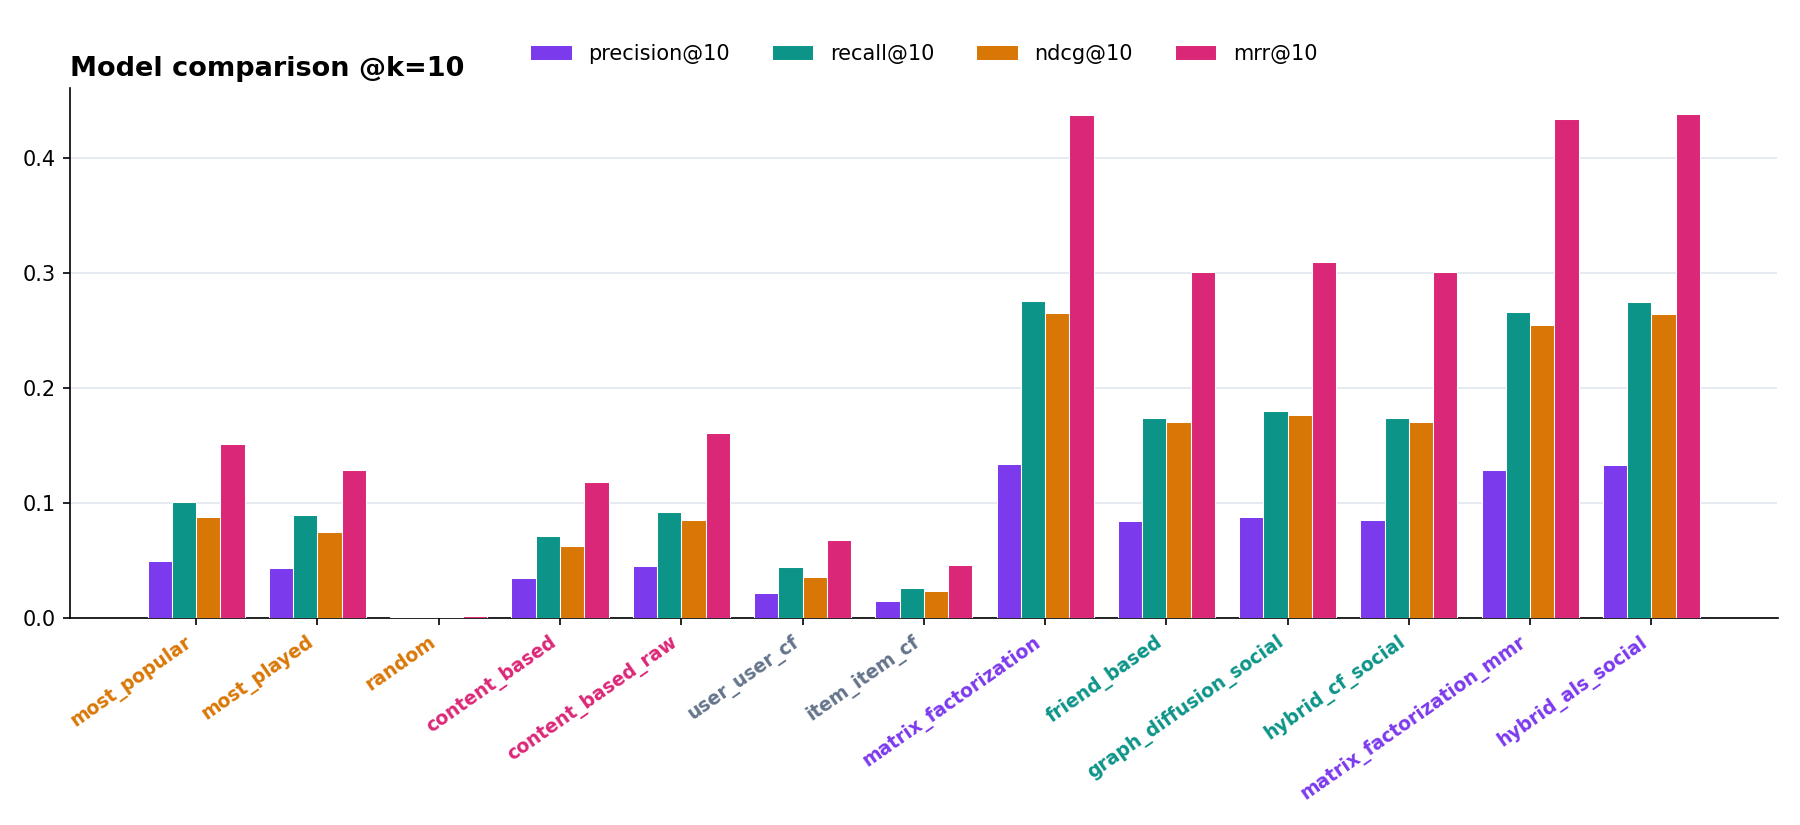
\includegraphics[width=\linewidth]{results/figures/metrics_comparison.png}
\caption{Accuracy metrics @k=10 across all 13 models.}
\end{figure}

\subsection{Headline finding: implicit ALS wins on every accuracy metric, by a wide margin}

Over 2.7x Most Popular's precision. This is backed by both significance testing and multi-seed variance, not just one split's numbers: a paired Wilcoxon signed-rank test on per-user NDCG@10 rejects the null at $p \approx 1.9 \times 10^{-79}$ (ALS vs.\ Friend-Based) and $p \approx 9.8 \times 10^{-183}$ (ALS vs.\ Most Popular); across 5 random train/test splits, ALS's precision@10 is $0.1336 \pm 0.0022$ vs.\ Friend-Based's $0.0876 \pm 0.0020$, a gap roughly 10x the combined standard deviation, i.e.\ not remotely explainable by which 20\% of each user's history happened to land in the test set (\code{results/metrics\_multiseed\_summary.csv}).

\subsection{ALS's accuracy win comes with a hidden cost}

It is also one of the most popularity-biased personalized models (0.992), nearly as biased as Most Popular itself (1.000), with the lowest novelty (4.05) and lowest catalog coverage (0.039) of any non-trivial model. This is the single most important ``accuracy is not enough'' finding in this report. ALS's implicit-feedback objective is trained with confidence weights proportional to play count, and popular artists accumulate plays from many users, so the model has disproportionately more signal to fit popular artists well, and disproportionately little to say about the long tail. Friend-Based, by contrast, gets to 63\% of ALS's precision at a meaningfully lower popularity bias (0.945) and over 4x its coverage (0.165 vs.\ 0.039): it's a more \emph{balanced} recommender even though it's a less \emph{accurate} one. Which model is actually ``better'' now depends on what the product is optimizing for, which is exactly the point the assignment's ``accuracy is not enough'' framing is making.

\begin{figure}[!htbp]
\centering
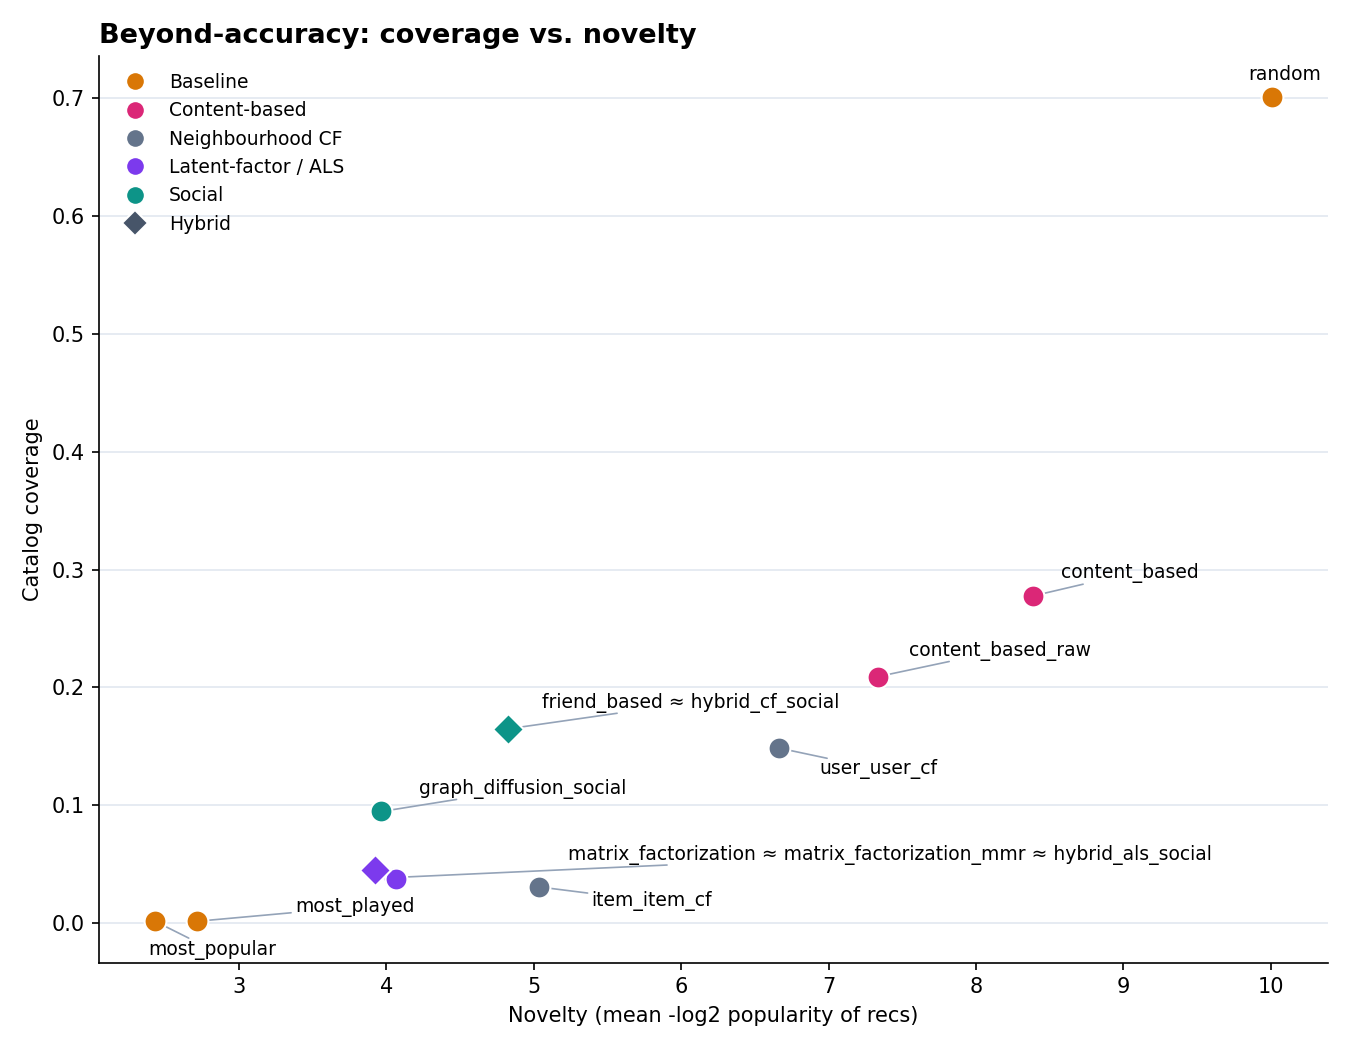
\includegraphics[width=0.85\linewidth]{results/figures/coverage_vs_novelty.png}
\caption{Beyond-accuracy: catalog coverage vs.\ novelty, colored by algorithm family.}
\label{fig:covnov}
\end{figure}

\subsection{Item-Item CF is similarly popularity-biased}

Despite the debugging story (\secref{sec:discussion}) being framed around it surfacing too-obscure artists, Item-Item CF's popularity bias is 0.983. The fix for that bug, a hard minimum-co-occurrence floor, has a side effect that isn't visible from the bug fix alone: it doesn't just suppress \emph{spurious} similarity estimates, it structurally excludes any artist too obscure to ever clear the floor from being recommended \emph{at all}. The bug fix traded ``occasionally nonsensical long-tail recommendations'' for ``systematic, structural exclusion of the long tail'': a real trade-off, not a clean win, that only became visible once the popularity-bias metric was added.

\subsection{The same trade-off shows up a third time, in the social layer}

Extending Friend-Based's reach from direct friends to a Personalized-PageRank-weighted neighbourhood (Graph Diffusion, \secref{sec:social}) raises precision@10 from 0.0845 to 0.0875 (+3.5\% relative) and NDCG from 0.1701 to 0.1764, a real, statistically significant gain (Wilcoxon $p \approx 0.011$), though a much smaller effect than the headline ALS comparisons. But every beyond-accuracy metric gets worse: coverage drops from 0.165 to 0.095 ($-42\%$), novelty from 4.83 to 3.97, diversity from 0.701 to 0.644, and popularity bias rises from 0.945 to 0.975, nearly as biased as Implicit ALS itself. This is the exact same story as the two sections above, Implicit ALS vs.\ Item-Item CF, replayed in a different layer of the same project: borrowing statistical strength from a wider neighbourhood (the whole interaction matrix for ALS, a multi-hop social neighbourhood for Graph Diffusion) buys real accuracy, and the price is a consistent drift toward the catalog's popular head; the neighbourhood that's doing the ``borrowing'' is, on average, more mainstream than any one user's direct connections. Three independent algorithm families converging on the same trade-off is much stronger evidence for it than any one result alone would be.

\begin{figure}[!htbp]
\centering
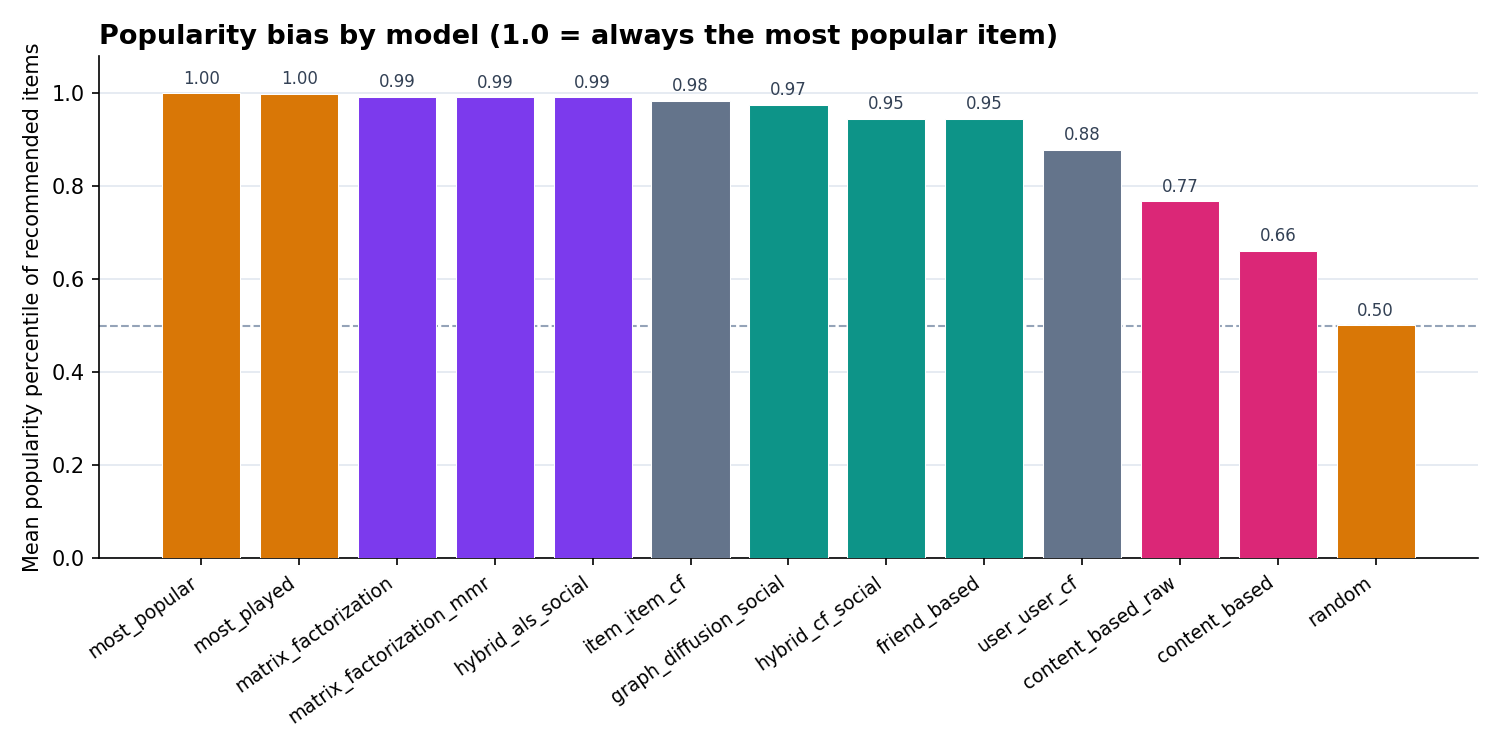
\includegraphics[width=0.85\linewidth]{results/figures/popularity_bias.png}
\caption{Popularity bias by model.}
\end{figure}

\subsection{ALS factor tuning produced this project's cleanest tuning win, and CF \texorpdfstring{$k$}{k} tuning its clearest non-result}

$n_{\text{factors}}=20$ beats the originally hand-picked $n_{\text{factors}}=50$ on validation NDCG (0.1904 vs.\ 0.1784), and that improvement \emph{carried over} cleanly to the held-out test set (precision@10 rose from 0.1312 to 0.1345): concrete evidence the original default was never actually checked. Item-item-CF $k$ tuning, by contrast, found validation NDCG is essentially flat across $k \in \{10,20,30,50\}$ (0.0255--0.0256, no meaningful difference): $k$ isn't the bottleneck for this algorithm on this dataset, the minimum-co-occurrence floor is (\secref{sec:discussion}), so spending more neighbours doesn't help once that floor is already the binding constraint. A non-result from a properly-run search is still a result: it tells you where \emph{not} to spend further tuning effort.

\subsection{Tuning ALS's regularization and confidence scaling was a real but mixed result}

Unlike the clean win $n_{\text{factors}}$ tuning was: \secref{sec:protocol} grid-searched $\text{reg} \in \{0.01,0.05,0.1,0.3\}$ and $\alpha \in \{1.0,2.0,4.0,8.0\}$ after fixing $n_{\text{factors}}=20$, and validation NDCG@10 improved from 0.1904 to 0.1934 (+1.6\%) at $\text{reg}=0.01, \alpha=1.0$, \emph{less} regularization and \emph{less} aggressive confidence weighting than the original hand-picked defaults ($\text{reg}=0.1, \alpha=2.0$). On the held-out test set, that improvement partially transferred: NDCG@10 rose ($0.2638 \to 0.2650$) and MRR@10 rose more ($0.4332 \to 0.4383$), but precision@10 and recall@10 both \emph{fell} slightly ($0.1345 \to 0.1335$; $0.2775 \to 0.2756$), and catalog coverage dropped 19\% relative ($0.048 \to 0.039$) alongside a meaningful novelty drop ($4.19 \to 4.05$). A lower $\alpha$ means confidence scales less steeply with play count, which sounds like it should reduce popularity bias, not increase it ($0.990 \to 0.992$), but the metric this search optimized for is NDCG, which rewards getting the \emph{top few ranks} right more than it rewards spreading recommendations across the catalog, and apparently the validation split's top-rank-friendly optimum is one that leans harder on a smaller set of well-supported (= popular) artists. A small, real win on the metric being optimized, and a small, real cost on three metrics that weren't: exactly the kind of result the four separate beyond-accuracy metrics (\secref{sec:protocol}) exist to catch, rather than a single accuracy number hiding it.

\subsection{Hybrid weight tuning converged to a boundary optimum: 0\% CF / 100\% social}

Grid-searching the blend weight (\secref{sec:protocol}) on held-out validation NDCG@10 (not hand-picked, and not the test set) produced a strictly monotonic curve: \emph{every} increment of CF weight made validation NDCG worse, all the way down to 0:

\begin{table}[!htbp]
\centering
\begin{tabular}{rrr}
\toprule
Item-item CF weight & Friend-based weight & val NDCG@10 \\
\midrule
0.00 & 1.00 & 0.1351 \\
0.20 & 0.80 & 0.1307 \\
0.35 & 0.65 & 0.1218 \\
0.50 & 0.50 & 0.0968 \\
0.65 & 0.35 & 0.0817 \\
0.80 & 0.20 & 0.0588 \\
1.00 & 0.00 & 0.0278 \\
\bottomrule
\end{tabular}
\caption{CF/social hybrid weight grid search (validation NDCG@10).}
\end{table}

This is a real, useful finding, not a tuning failure: it's quantitative confirmation that on this dataset, once the social signal is available, item-item CF adds nothing, it's actively diluting a stronger signal, not complementing a weaker one. (The original hand-picked 0.65/0.35 weight \emph{favoured the weaker signal}, which in hindsight was backwards; see \secref{sec:discussion} for the full discussion, including a genuinely subtle implementation detail this discovery exposed.) A paired Wilcoxon test confirms Friend-Based and the tuned Hybrid are \emph{not} significantly different ($p=0.317$), consistent with the hybrid degenerating to friend-based at this weight (\secref{sec:discussion}).

\subsection{The ALS + Graph-Diffusion hybrid is this project's clearest example of validation-set overfitting}

Caught only because there's a separate held-out test set. \code{tune\_als\_social\_hybrid\_weight()} (\secref{sec:social}) is the natural follow-up to the CF+Social search above: does blending this project's two most accurate \emph{individual} models do any better than either alone? On validation it found a genuine interior optimum: 80\% ALS / 20\% Graph Diffusion beat pure ALS by $+1.1\%$ NDCG (0.1956 vs.\ 0.1934), a real non-boundary result, unlike the CF+Social hybrid's collapse to a 0\% weight. But on the held-out test set, the same blend is \emph{not} better than plain ALS: NDCG@10 0.2646 vs.\ 0.2650, precision@10 0.1327 vs.\ 0.1335, both very slightly worse, and a paired Wilcoxon test confirms this small gap is statistically significant ($p \approx 7.8 \times 10^{-5}$), not noise. In other words, the validation-set ``improvement'' was real \emph{on that specific 15\%-of-training slice}, but it doesn't generalize, and the failure to generalize is itself a robust, repeatable effect, not sampling variance in the test evaluation. The mechanism is almost certainly the 7-point weight grid searched against a validation set roughly an order of magnitude smaller than the test set: enough room for a blend to fit validation-specific noise in exactly the way a single hand-picked hyperparameter is less likely to. This is exactly why this project keeps the test set strictly separate from every tuning decision (\secref{sec:protocol}): without that separation, \code{hybrid\_als\_social} would have shipped as a quiet accuracy regression dressed up as an improvement.

\begin{figure}[!htbp]
\centering
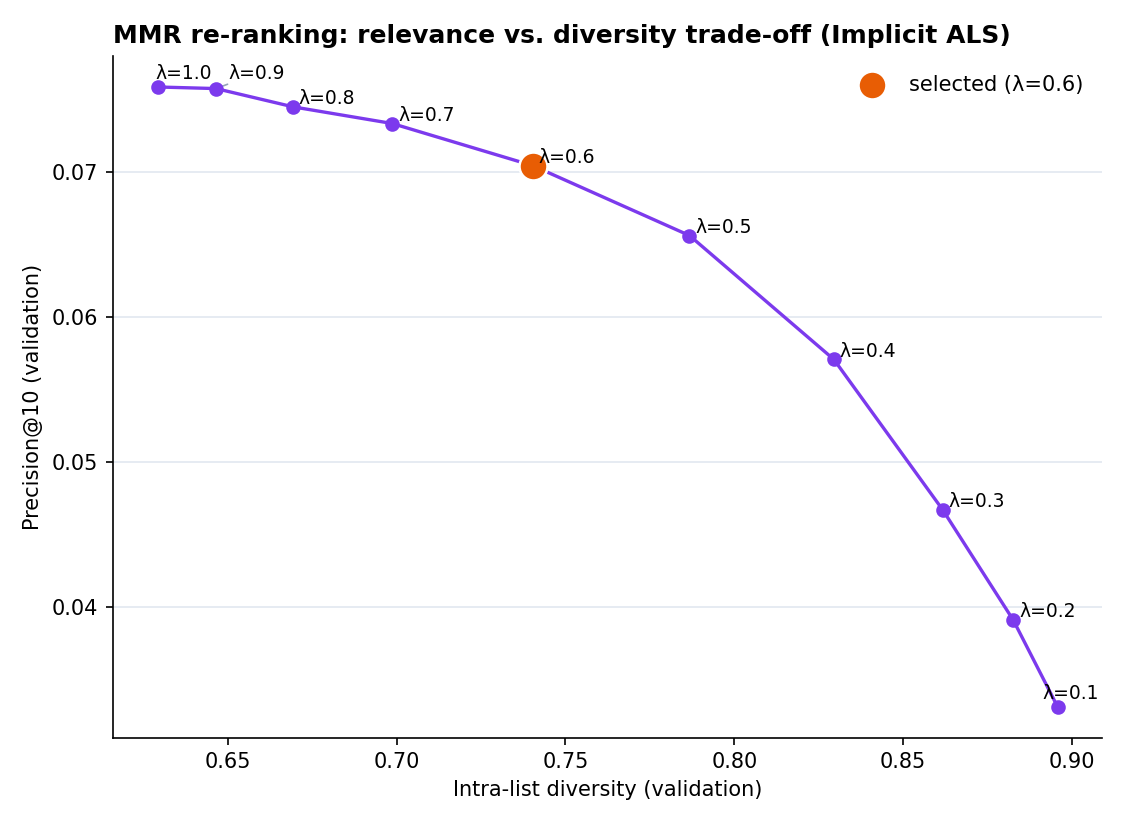
\includegraphics[width=0.7\linewidth]{results/figures/mmr_tradeoff.png}
\caption{MMR re-ranking: relevance vs.\ diversity Pareto curve (Implicit ALS).}
\label{fig:mmr}
\end{figure}

\subsection{MMR re-ranking fixes the metric it targets and only that metric}

A result that's more informative than a clean win would have been. On the held-out test set, ALS+MMR ($\lambda=0.6$) raises diversity from 0.637 to 0.742 (+16\%) at a statistically significant (Wilcoxon $p \approx 3.4 \times 10^{-14}$) but modest precision cost ($0.1335 \to 0.1285$, $-3.7\%$ relative; NDCG $-3.9\%$), close to the trade-off the validation sweep predicted choosing $\lambda$ this way, which is itself a useful confirmation that the inner-split tuning generalizes to the test set (unlike the ALS+social hybrid's weight, above). But popularity bias barely moves ($0.9919 \to 0.9916$) and coverage/novelty don't improve either (coverage $0.039 \to 0.038$, novelty $4.05 \to 4.07$): diversifying \emph{within} a list by tag-content dissimilarity is not the same lever as reducing \emph{how popular} the items in that list are, even though it would be easy to assume the two move together. They don't: a list can mix tag-dissimilar artists that are all still mainstream-popular, and MMR has no signal telling it otherwise since it only ever compares candidates to each other, not to a global popularity baseline. This is the same lesson \secref{sec:protocol} already drew from having four separate beyond-accuracy metrics instead of one; it just took building an actual mitigation to see it apply to a \emph{fix}, not only to a \emph{measurement}. (One more real cost, not in the table: MMR's greedy per-candidate cosine-similarity loop makes evaluation $\sim$88x slower than plain ALS, 175s vs.\ 2.0s for 1{,}874 users, a latency trade-off that would matter for an online re-ranking deployment, not just an offline metric.)

\subsection{The headline model ranking does not depend on the specific choice of relevance threshold}

Every ranking metric in this report rests on one specific definition of ``relevant'' (held-out play count $\geq$ the user's training median, \secref{sec:protocol}). \code{relevance\_threshold\_check.py} re-evaluated six representative models under three definitions, ``any play counts'' ($q=0.00$), the project default ($q=0.50$), and a stricter ``favourite-tier only'' bar ($q=0.75$), and the precision@10 ranking across all six models is identical at every threshold: Implicit ALS first, Graph Diffusion second, Friend-Based third, Most Popular fourth, Content-Based (raw) fifth, Item-Item CF last. The absolute numbers move a lot with the threshold (e.g.\ ALS's P@10 ranges from 0.193 at $q=0.00$ down to 0.093 at $q=0.75$, since a stricter bar makes every list harder to hit), but \emph{which model wins} never changes: the comparative conclusions in this report aren't an artifact of where exactly the relevance bar was set.

\subsection{TF-IDF vs.\ raw tag counts: the simpler model wins on accuracy, the fancier one wins on everything else}

Raw counts beat TF-IDF on every ranking metric (precision@10 0.0449 vs.\ 0.0344, +30\% relative) but TF-IDF wins on coverage (0.278 vs.\ 0.209) and novelty (8.39 vs.\ 7.33), and both have nearly identical diversity ($\sim$0.32). The likely explanation: TF-IDF's whole point is down-weighting tags that are common across many artists (e.g.\ ``rock'', ``electronic''), but for this dataset, those broad genre tags are themselves a big part of what makes two artists actually similar in a way that predicts shared listeners, while the rare tags TF-IDF up-weights in exchange are often one-off, idiosyncratic taggings that don't generalize. This is a useful, slightly humbling result: a standard NLP weighting trick doesn't automatically transfer just because the technical analogy (artist tags $\approx$ document terms) is appealing.

\subsection{The diversity column tells a story accuracy alone hides}

Both Content-Based variants have by far the lowest diversity ($\sim$0.32) of any non-trivial model: they're explicitly built to find tag-cosine-similar items, so their top-10 for any user clusters tightly in tag-space (e.g.\ all trip-hop, all neo-classical, see \secref{sec:examples}). Random sits at the opposite extreme (0.990) precisely because it has no notion of ``similar'' at all.

\subsection{Most Popular is a deceptively strong baseline}

Common in implicit recommender literature, and visible here too: popularity bias means ``recommend whatever's universally liked'' scores reasonably on raw accuracy. Its near-zero coverage (0.002) and low novelty (2.4) make clear why it's not a \emph{good} recommender despite the score; this is exactly what the beyond-accuracy metrics are for. Random's popularity bias of 0.501 is a useful sanity check on the metric itself: a model with literally no preference for popular items should land almost exactly at the 50th percentile, and it does.

\section{Recommendation examples}
\label{sec:examples}

Full output for 3 users (with $\geq$3 friends, so the social layer has something to show) is in \code{results/examples/recommendation\_examples.txt}. One representative case, User 2 (40 training artists):

\begin{table}[!htbp]
\centering
\small
\begin{tabular}{lp{9.5cm}}
\toprule
Model & Top picks \\
\midrule
Most Popular & Britney Spears, The Beatles, Rihanna, Katy Perry \\
Content-Based (TF-IDF) & Massive Attack, Portishead, Emancipator, J.Viewz \\
Content-Based (raw) & Massive Attack, T\'el\'epopmusik, Moby, Everything but the Girl \\
Item-Item CF & Yazoo, Gary Numan, Eurythmics, Ultravox, The Human League \\
Implicit ALS (tuned) & Pet Shop Boys, U2, R\"oyksopp, Michael Jackson, Moby \\
Friend-Based & Pet Shop Boys, Michael Jackson, Simple Minds, Erasure \\
Graph Diffusion (PPR) & Pet Shop Boys, The Cure, Michael Jackson, The Human League, Erasure \\
Hybrid (CF+social, 0/1) & Pet Shop Boys, Michael Jackson, Simple Minds, Erasure \\
Hybrid (ALS+GD, 0.8/0.2) & Pet Shop Boys, U2, R\"oyksopp, Michael Jackson, Moby \\
\bottomrule
\end{tabular}
\caption{Recommendation examples for User 2.}
\end{table}

This is a satisfying result to read by eye: Item-Item CF, ALS, and the friend-based recommender all independently converge on \emph{80s synth-pop/new-wave} (Pet Shop Boys, Yazoo, Eurythmics, Simple Minds, The Human League) for this user, while both Content-Based variants, working from a much sparser tag signal, land on trip-hop/downtempo instead (Massive Attack, Portishead, T\'el\'epopmusik, Moby). Three structurally different algorithms agreeing is good evidence that the agreement reflects the user's actual taste rather than each model independently latching onto noise; the two Content-Based variants agreeing with \emph{each other} but not the rest is consistent with \secref{sec:results}'s finding that they're measuring something correlated with each other (the same tag corpus) but not as strongly correlated with actual held-out listening as the behaviour-based signals are. Graph Diffusion lands in the same 80s synth-pop cluster as Friend-Based, plus one extra pick (The Cure) that direct friends alone didn't surface: a small, concrete illustration of \secref{sec:results}'s finding that extending the social reach trades some specificity for a wider net. The Hybrid (CF + social) row is now \emph{identical} to Friend-Based for this user, the direct, visible consequence of the tuned 0.00/1.00 weight discussed in \secref{sec:results} and \secref{sec:discussion}: with zero weight on CF, the only way the hybrid can differ from pure friend-based is for a user whose friend list is empty (where CF still acts as a fallback list, see \secref{sec:discussion}). The Hybrid (ALS + Graph Diffusion) row is, for this particular user, \emph{identical} to plain Implicit ALS, a small concrete preview of \secref{sec:results}'s finding that the 80/20 blend doesn't meaningfully move the needle on test-set recommendations despite its validation-set ``win''.

\section{Discussion, debugging story, and limitations}
\label{sec:discussion}

\subsection{The debugging story}

Worth documenting because it changed the final design. The first working version of item-item CF recommended almost exclusively obscure 5--10-listener artists, with near-zero precision (0.0002). Root cause: the prediction formula
\begin{equation}
\text{score}(u,i) = \frac{\sum_j \text{sim}(i,j) \cdot \text{val}(u,j)}{\sum_j |\text{sim}(i,j)|}
\end{equation}
is a \emph{weighted average}, and when only one neighbour $j$ passes the top-$k$ cut for a given candidate $i$, the similarity magnitude cancels out of the ratio entirely, so the prediction collapses to ``whatever the user's play value was for that one neighbour,'' regardless of how small or statistically meaningless the similarity actually was. Combined with a median of 1 listener per artist, this meant a single coincidental overlap could hijack the top of a recommendation list. The fix was a hard co-occurrence floor: similarity pairs backed by fewer than \code{min\_co\_count} shared listeners (tuned separately for item-item vs.\ user-user; items need a looser floor than users here, since user-user shared-artist support is much harder to come by) are zeroed out entirely, on top of the existing ``shrinkage'' soft correction ($\text{co\_count}/(\text{co\_count}+\beta)$, \citealp{sarwar2001item}). After the fix, Item-Item CF's example recommendations are genre-coherent (see \secref{sec:examples}) even though its aggregate metrics are still modest; see below.

\subsection{Why does CF still lag ALS and the social layer so much, even after the fix?}

With only $\sim$5 listeners per artist on average and a strict minimum-support floor, the \emph{evaluable} item-item neighbourhood is much smaller than the full catalog (a large share of artists never clear the co-occurrence floor at all), so CF's coverage and reach are intrinsically limited on a dataset this sparse: exactly the scenario latent-factor models are designed to handle better, since ALS can borrow statistical strength across the \emph{whole} matrix rather than only from artists with directly-overlapping listeners.

\subsection{Why did the validated hybrid weight collapse to 0\% CF?}

\secref{sec:results}'s grid-search table shows the curve is strictly monotonic, not just minimized at an interior point: every unit of weight moved from social to CF made validation NDCG worse. The likely reason is the same one from the debugging story above: item-item CF's effective neighbourhood, after the necessary minimum-support floor, only covers a fraction of the catalog on this sparse dataset, so it has comparatively little to contribute once a much stronger, much broader signal (the friend graph) is already in the blend, there's no ``second opinion'' benefit if the second opinion is mostly noise relative to the first. This reverses the original (hand-picked, 0.65/0.35-weighted) version of this project's conclusion, which is the point of tuning empirically rather than asserting a blend ratio: the original weighting happened to favour the \emph{weaker} of the two signals.

\subsection{A genuinely subtle finding the tuning exposed}

At the validated 0.00/1.00 weight, the hybrid still edges out pure Friend-Based by a hair (P@10 0.0846 vs.\ 0.0845, see \secref{sec:results}), which looks like it shouldn't be possible, since a weight of exactly 0 means item-item CF's reciprocal-rank contribution ($\text{weight}/(\text{rank}+1)$) is \emph{mathematically} zero for every rank. The reason: \code{HybridRecommender}'s fusion adds each model's zero-valued candidates to the score dict regardless, and Python's \code{sorted()} is stable, so when a user has no friends (friend-based contributes nothing) but does have CF neighbours, those candidates survive the merge in their \emph{original} CF rank order purely through insertion-order tie-breaking, not because their score reflects that order. It works here, but it's an implementation accident, not a designed fallback: a more deliberate version would special-case ``this component contributed only zero-scored candidates'' into an explicit secondary ranking rather than relying on dict/sort stability.

\subsection{Cold-start backfill: before vs.\ after}

Wrapping the four models that had $n_{\text{users\_no\_recs}} > 0$ with \code{BackfillRecommender} (Most-Popular top-up) and re-evaluating gives a direct before/after read on the trade-off (\code{results/metrics\_backfilled.csv}):

\begin{table}[!htbp]
\centering
\begin{tabular}{lrrr}
\toprule
Model & P@10 (raw) & P@10 (backfilled) & no-recs (raw $\to$ backfilled) \\
\midrule
Content-Based & 0.0344 & 0.0344 & 2 $\to$ 0 \\
User-User CF & 0.0210 & 0.0227 & 346 $\to$ 0 \\
Item-Item CF & 0.0141 & 0.0139 & 33 $\to$ 0 \\
Friend-Based & 0.0845 & 0.0845 & 0 $\to$ 0 \\
\bottomrule
\end{tabular}
\caption{Cold-start backfill before/after comparison.}
\end{table}

User-User CF's accuracy \emph{improves} after backfill: its 346 no-rec users (18\% of the evaluable set) were contributing zero precision either way, so giving them Most-Popular's reasonably-strong baseline picks instead of nothing is a strict improvement. Item-Item CF dips by 0.0002 (33 users, 1.8\%): negligible, and within noise for a single split. This is why the backfilled numbers are reported separately rather than replacing \secref{sec:results}'s table: for the \emph{algorithm comparison}, the raw numbers are the honest ones; for the \emph{product} (\secref{sec:prototype}), backfilled is strictly better UX for a near-zero accuracy cost.

\subsection{Temporal split check: is the random-split headline optimistic?}

\secref{sec:results}'s results all use a per-user \emph{random} 80/20 split, which isn't a strict ``predict the future from the past'' evaluation. A genuine temporal split turns out not to be straightforwardly possible on this dataset: \code{user\_artists.dat} (the play-count data every model trains on) carries no timestamp at all. The only timestamp anywhere in HetRec2011 is on tag-application events, and only 22.3\% of (user, artist) listening interactions even have one (\code{data\_loading.get\_interaction\_timestamps}, using each pair's earliest tag date as a proxy ``interaction time'').

\code{temporal\_split\_check.py} makes the best of that constraint: it restricts \emph{both} a random split and a temporal split to exactly the same 20{,}665 timestamped interactions (1{,}824 users), so the only thing that differs between the two conditions is \emph{which} of a user's interactions get held out, not how much data the models see. Most Popular and Implicit ALS, refit on this reduced data under each condition:

\begin{table}[!htbp]
\centering
\begin{tabular}{llrrr}
\toprule
Split & Model & P@10 & R@10 & NDCG@10 \\
\midrule
Random & Most Popular & 0.0210 & 0.1043 & 0.0664 \\
Random & Implicit ALS & 0.0497 & 0.2220 & 0.1636 \\
Temporal & Most Popular & 0.0125 & 0.0702 & 0.0456 \\
Temporal & Implicit ALS & 0.0233 & 0.1322 & 0.0815 \\
\bottomrule
\end{tabular}
\caption{Random vs.\ temporal split, restricted to timestamped interactions only. Not comparable in absolute magnitude to Table~\ref{tab:results}, this fits on $\sim$22\% of the data.}
\end{table}

Two findings. First, the random split is optimistic for both models: NDCG drops 31\% for Most Popular and 50\% for Implicit ALS once the test set is genuinely ``the future'' instead of a random hold-out, confirming the suspicion that prompted this check. Second, and more interesting: ALS's relative advantage over Most Popular shrinks under temporal evaluation, 2.46x under random split (0.1636 vs.\ 0.0664) but only 1.79x under temporal split (0.0815 vs.\ 0.0456). Some of what looks like ``ALS is much better at personalization'' in \secref{sec:results} is partly ``ALS is better at exploiting patterns that a random hold-out doesn't punish as harshly as genuinely new, future listening would'': a real result, even though the data only supports checking it on a 22\% subset. ALS still clearly wins both ways, so the headline conclusion of \secref{sec:results} stands; the \emph{size} of the win is the part this check tempers.

\subsection{Limitations}

\begin{itemize}[leftmargin=*]
  \item Every recommendation in this project is artist-level, not song-level (\secref{sec:dataset}): \code{user\_artists.dat} has no track-level data to fall back to, so this isn't a modeling choice that could be fixed within HetRec2011, it's a property of the dataset itself. MSD Taste Profile or Spotify MPD would give song-level recommendations directly, at the cost of HetRec2011's tag and social layers (\secref{sec:dataset}). The live product (\secref{sec:prototype}) papers over this cosmetically, a per-card top-track lookup, without changing what's actually being recommended.
  \item The temporal split check is necessarily partial (22.3\% interaction coverage, and a tag-date proxy rather than a true listen date): a dataset with real interaction timestamps (e.g.\ MSD Taste Profile) would let this be done properly across 100\% of the data, not as a scoped add-on.
  \item The hybrid's zero-weight fallback behaviour is incidental, not designed (see above): it happens to work due to stable-sort insertion order, which is a fragile thing to depend on.
  \item Backfill is applied at the UI layer only: \code{main.py}'s headline evaluation table intentionally reports unmodified per-algorithm accuracy; a deployed system would likely want every model backfilled by default, which would mean re-deciding whether backfilled or raw numbers are the ``real'' comparison for model selection.
  \item MMR re-ranking (\secref{sec:mmr}/\secref{sec:results}) fixes ALS's low intra-list diversity but not its popularity bias, coverage, or novelty: ``diversity'' and ``popularity bias'' turn out to be independent enough that one technique addressing one doesn't fix the other; a production system that wants \emph{all four} beyond-accuracy properties improved would need a re-ranking objective that explicitly penalizes popularity, not just tag-content redundancy.
  \item MMR's greedy per-candidate re-ranking is $\sim$88x slower than plain ALS scoring at evaluation time (\secref{sec:results}): fine for a request-time re-rank of a fixed-size candidate pool (as \code{backend/}'s feedback loop, \secref{sec:prototype}, already does for a different fusion), but the gap would matter more at a larger pool size or stricter latency budget than this prototype has.
  \item \code{reg}/$\alpha$ were staged after $n_{\text{factors}}$ rather than searched jointly (\secref{sec:protocol}) to keep the grid small (16 fits instead of 48): it's possible $n_{\text{factors}}=50$ or $80$ would prefer a different \code{reg}/$\alpha$ than $n_{\text{factors}}=20$ does, and a joint search would catch that; this wasn't tested, the same trade-off \code{tune\_model\_params()}'s staged design already makes for $k$ vs.\ the hybrid weight.
  \item Only one of this project's five tuned hyperparameters/weights was directly shown to overfit its validation split (the ALS+Graph-Diffusion hybrid weight, \secref{sec:results}): that doesn't mean the other four ($n_{\text{factors}}$, CF $k$, the CF+Social weight, MMR's $\lambda$) are \emph{guaranteed} clean; it means their validation-set ``wins'' happened not to reverse on this particular test set. A single 85/15 inner split, reused for five separate searches, is enough to catch \emph{a} validation-overfit when one occurs (as it did here) but isn't a guarantee against a subtler one in any of the others; repeated/nested cross-validation across multiple inner splits would give a more complete picture, at proportionally more compute cost.
  \item Item-item-CF $k$ tuning searched a fairly coarse grid ($\{10,20,30,50\}$) and found it doesn't matter much in that range: it's possible a much smaller $k$ (e.g.\ 3--5) would behave differently, since the minimum-co-occurrence floor already does most of the filtering work; this wasn't tested.
  \item Graph Diffusion's restart probability (0.15) and neighbour cap (100) are the conventional PageRank defaults, not grid-searched on this dataset, the way $n_{\text{factors}}$, CF $k$, the hybrid weight, and MMR's $\lambda$ all are (\secref{sec:protocol}). Unlike those four, this one parameter was deliberately left at a standard, well-studied value rather than tuned, so it's possible a dataset-specific restart probability would shift \secref{sec:results}'s accuracy/popularity-bias trade-off in either direction.
\end{itemize}

\section{Conclusion}
\label{sec:conclusion}

Switching to the Last.fm track over MovieLens paid off specifically because the dataset's extra layers (tags, friend graph) let the project demonstrate genuinely different recommendation paradigms, content-based, neighborhood CF, latent-factor, and social, on the \emph{same} users, and directly compare how much each layer adds. The clearest takeaways:

\begin{enumerate}[leftmargin=*]
  \item Matching the algorithm to the feedback type matters enormously: implicit ALS vs.\ naive SGD would have been the wrong tool entirely.
  \item A recommender's social graph, where available, is a remarkably strong signal on its own, beating every similarity-based CF variant here, and statistically indistinguishable from a hybrid that's supposed to improve on it ($p=0.317$, \secref{sec:results}) once the blend weight is tuned rather than guessed.
  \item Low-support similarity estimates need explicit statistical guardrails on sparse implicit data, or they silently produce nonsense recommendations that look fine until you actually read them, but the guardrail itself has a cost (\secref{sec:results}, \secref{sec:discussion}): it trades spurious long-tail noise for \emph{structural} long-tail exclusion, raising popularity bias as a side effect invisible without a dedicated metric.
  \item A hybrid's blend weight, and a latent-factor model's factor count, should be \emph{validated}, not asserted. Grid-searching both on held-out data reversed this project's own earlier (hand-picked) hybrid-weight conclusion, and found the original ALS factor count was never actually a good choice for this dataset (\secref{sec:results}).
  \item The most accurate model is not the most balanced one, and you only find that out by measuring more than accuracy. Implicit ALS wins precision/recall/NDCG by a wide, statistically-significant, seed-robust margin (\secref{sec:results}), and is simultaneously one of the two most popularity-biased, least novel personalized models in the whole comparison. Neither fact is more ``true'' than the other; a real product decision here depends on what's actually being optimized for.
  \item A standard technique transferring by analogy doesn't mean it transfers in practice: TF-IDF down-weighting ``common'' terms is exactly the right move for text documents, and exactly the wrong default assumption for this dataset's tags, where raw counts won on every accuracy metric (\secref{sec:results}).
  \item Beyond-accuracy metrics aren't fungible, and neither are the fixes for them. Adding an actual mitigation (MMR re-ranking, \secref{sec:mmr}) for the model's worst-measured weakness raised diversity 16\% at a real but bounded precision cost, and left popularity bias, coverage, and novelty essentially untouched, even though all four are usually discussed together as ``the beyond-accuracy story.'' Measuring four distinct things and then building a fix for only one of them is what exposed that they don't move together.
  \item The accuracy/popularity-bias trade-off isn't specific to matrix factorization, it's what happens whenever a model borrows statistical strength from a wider neighbourhood, and this project found the same pattern three times, across both layers it has: Implicit ALS and Item-Item CF in the listening layer, and Graph Diffusion vs.\ Friend-Based in the social layer (\secref{sec:results}). Three largely independent results landing on the same trade-off is much stronger evidence for a general principle than any one of them alone would be.
  \item A headline conclusion is only as strong as the assumptions it quietly rests on, so check the quiet ones too. The relevance threshold (\secref{sec:protocol}/\secref{sec:results}) is one specific, otherwise-unexamined design choice; re-running the comparison under two very different alternative definitions left the model ranking completely unchanged, which is exactly the kind of check that's cheap to skip and easy to regret skipping.
  \item Validating a hyperparameter on held-out data is necessary, but it is not the same thing as proving it generalizes: only a separate, untouched test set can show the difference. This project tuned five hyperparameters/weights on the same inner validation split (\secref{sec:protocol}); four of those validation-set ``wins'' held up on the held-out test set, and one, the ALS+Graph-Diffusion hybrid weight, didn't: it beat plain ALS by +1.1\% on validation and lost to it, \emph{significantly}, on test (\secref{sec:results}). That reversal is only visible \emph{because} the test set was kept strictly separate from every tuning decision; a project that tuned directly against its reported numbers would have shipped that regression as an improvement and never known.
\end{enumerate}

Across ten algorithms spanning three data layers, six tuned hyperparameters, and the significance, multi-seed, temporal, and relevance-threshold checks in \secref{sec:protocol}/\secref{sec:discussion}, the throughline is the same one the assignment's own ``accuracy is not enough'' framing points at: a single number is never the full story, every claim of ``better'' needs a stated metric and a test for whether the gap is real, and a held-out set that's never touched during tuning is what turns ``we think this works'' into ``we checked.''

\section{Interactive prototype}
\label{sec:prototype}

\subsection{Architecture}

The first iteration of the prototype was a single Streamlit script that doubled as both a product demo and a research dashboard: recommendation cards next to model names, accuracy tables, and algorithm explanations on the same screen. That's the right tool for \emph{this report's} analysis, but the wrong one for a user-facing product, so the prototype was rebuilt as two separate pieces:

\begin{itemize}[leftmargin=*]
  \item \code{backend/}: a small FastAPI service. On startup it fits Most Popular, content-based (raw counts), implicit ALS ($n_{\text{factors}}=20$, the validated value from \secref{sec:results}), and the friend-based recommender once, on the \emph{full} interaction history (not the 80/20 split, a live product should use every bit of signal it has, there's no test set to protect). It exposes endpoints for a listener list (for the switcher), a random listener, and a single \code{/api/home/\{id\}} endpoint that returns one listener's whole home feed in one call. It intentionally keeps ALS's original $\text{reg}=0.1, \alpha=2.0$ rather than the later-tuned $\text{reg}=0.01, \alpha=1.0$ (\secref{sec:results}): that tuning's test-set effect was a genuine mixed trade (NDCG/MRR up, precision/coverage/novelty down), not a clean win, so there's no obviously-correct choice to ship to the product without first deciding what ``Made For You'' should optimize for, exactly the kind of decision \secref{sec:results} flags as depending on what's being optimized, not resolved by it.
  \item \code{frontend/}: a React + Tailwind single-page app (``Wavelength''), a dark, card-based layout deliberately closer to a consumer music app than a research tool.
\end{itemize}

The product deliberately keeps \code{FriendBasedRecommender}, not Graph Diffusion (\secref{sec:social}/\secref{sec:results}), behind ``Friends Are Listening To'' even though Graph Diffusion is the more accurate of the two: that shelf's name is a literal promise (``your friends are listening to this''), and Graph Diffusion's recommendations come partly from friends-of-friends, which would make the label inaccurate. A product that wanted to surface Graph Diffusion's accuracy gain would need a shelf that doesn't over-promise about \emph{whose} listening produced the picks: a UX naming problem, not a modeling one.

\subsection{What the user sees, and what they don't}

Every technical detail in this report (model names, scores, coverage/novelty/diversity numbers, the debugging story) is absent from the UI on purpose. A listener picks or shuffles to a user ID (HetRec's users are anonymized IDs with no profile data to log in with, so switching listener = switching ``account'' for demo purposes) and sees four shelves: \emph{Made For You} (implicit ALS), \emph{Friends Are Listening To} (the friend-based recommender, framed as what it actually is rather than as ``social filtering''), \emph{Because You Listened To \texttt{<artist>}} (content-based similar-artists, seeded on whichever of the listener's top artists has the richest tag coverage), and \emph{Trending Now} (Most Popular). The mapping from UI section to underlying model exists only in this report and in \code{backend/recommender\_service.py}'s comments, not anywhere a user can see it. This was a deliberate scope decision: the assignment's evaluation/comparison work and the product experience are different deliverables with different audiences, and conflating them (numbers and jargon on a consumer screen) would have hurt both.

\subsection{Cold-start, invisibly}

\secref{sec:backfill}/\secref{sec:discussion} already established that backfilling short lists with Most-Popular picks is a near-zero-cost fix for empty results. The research prototype marked backfilled items with a pin icon for transparency; the product prototype does the same backfill but shows nothing, a real listener doesn't need to know which of their recommendations came from a fallback.

\subsection{Artist artwork}

The dataset's own \code{pictureURL} column points at a 2011-era Last.fm CDN domain that no longer resolves (verified by DNS lookup, not assumption). Real artwork is instead fetched live, per artist, from the iTunes Search API (\code{backend/artist\_images.py}), keyless, no account setup, and cached to disk so repeat lookups are instant. Any artist with no match, or a failed image load in the browser, falls back to a deterministic gradient avatar (a hash of the artist's name picks the colors), the same pattern Slack/Spotify use for entities without a photo, so a flaky network or an obscure artist never produces a broken-image icon.

\subsection{Track titles}

These don't change what \secref{sec:dataset}/\secref{sec:discussion} already say. Every card also shows a representative track title under the artist name, resolved live from Deezer's public API (cached to disk, absent if no match), chosen over iTunes Search (used for artwork above) because Deezer has an actual artist-top-tracks endpoint ranked by real popularity, rather than relying on a relevance-ranked search query for a song; it also turned out to have a far more generous, reliable rate limit in practice than iTunes' for this query shape. This exists purely so the UI doesn't read as a bare list of artist names; it does \emph{not} mean the product recommends songs: the underlying ranking is still produced entirely by artist-level models (\secref{sec:dataset}), and the displayed track is not chosen by, or scored by, any recommender in this project. It is a cosmetic label, not a different granularity of recommendation, and is presented as such here rather than silently implying otherwise.

\subsection{Browsing into song granularity, deliberately, at the UI layer only}

Clicking an artist card's avatar opens a popup listing that artist's top 10 tracks (same Deezer lookup as above, just not truncated to one, plus a 30-second preview playable via a persistent mini-player). From there a listener can add individual tracks to any number of named, listener-created playlists; a track can belong to several at once, playlists are created inline from the same ``add to playlist'' menu, and a ``Playlists'' button in the header lists/opens/deletes them, separate from the artist-level like/skip that drives ``Made For You'' re-ranking below. This is the honest version of ``act on songs'' given the dataset constraint in \secref{sec:dataset}: the \emph{recommending} is still entirely artist-level (nothing about which tracks appear, which artist got recommended in the first place, or which playlist a listener builds is influenced by song-level data, because none exists in HetRec2011), but once a listener is looking at one already-recommended artist, letting them curate at song granularity costs nothing and doesn't misrepresent what the underlying models did. Playlists are stored separately from artist feedback (\code{data/processed/user\_feedback.json}'s \code{playlists}, keyed per listener) and don't feed back into any recommender, they're a personal collection, not a training signal.

\subsection{Feedback loop (like / skip)}

Every card has a heart and an X icon on hover. A skip is unconditional and immediate: the artist is filtered out of every shelf for that listener, both optimistically in the browser (instant) and on the next fetch from the backend (permanent, persisted to \code{data/processed/user\_feedback.json}). A like is more interesting: it does \emph{not} retrain anything, re-fitting implicit ALS per click is far too slow for an interactive UI. Instead, \code{recommender\_service.py}'s \code{\_made\_for\_you\_cards} re-ranks the existing ALS list with a reciprocal-rank-fusion blend (0.7/0.3) against the content-based similar-artists of everything the listener has liked so far, the same fusion technique \code{src/social\_filtering.py} uses for the offline CF+social hybrid (\secref{sec:social}), applied here as a cheap, request-time re-ranking layer on top of a statically-trained model rather than a retrain. The frontend debounces a home-feed refetch $\sim$700ms after each like/skip so a burst of clicks produces one visible update, not a flicker per click. This was validated end-to-end: liking a classic-rock artist from ``Trending Now'' visibly pulled several other classic-rock artists into ``Made For You'' on the next refetch, and a skipped artist disappeared from every shelf and did not reappear.

\subsection{Running it}

See \code{README.md}: \code{uvicorn backend.main:app} plus \code{npm run dev} in \code{frontend/}, two processes, no build step required for local use.

\subsection{Deployment}

Live at \url{https://13.49.21.10.nip.io}. Both services run on a single AWS EC2 instance (\code{t3.micro}, 1 vCPU, 1GB RAM) rather than on two separate platforms: Caddy serves \code{frontend/}'s static production build directly and reverse-proxies \code{/api/*} to the FastAPI backend on \code{127.0.0.1:8000}, so both are reached through the same origin. That choice wasn't the starting point; it's worth recording why, since it's a real example of a deployment decision driven by measurement rather than preference. The first attempt put the backend on Render's free tier (512MB) and the frontend on Vercel, the conventional split for a JS-frontend/Python-backend app. Render's free instance reliably OOM-killed the single worker process under real traffic on \code{/api/home/\{id\}}, the heaviest endpoint, since it resolves real artwork and track previews for every card in a request via two \code{ThreadPoolExecutor}s (the Artist artwork and Track titles sections above). This was confirmed directly, not inferred: Render's dashboard logs the exact event, \code{Ran out of memory (used over 512MB) while running your code}. Two rounds of trimming thread-pool concurrency (16 workers down to 3) and shelf size (12 items down to 8) reduced but did not eliminate the crashes: the four fitted models (ALS, content-based TF-IDF/count vectors, the interaction dataframe) already consumed a large share of the 512MB budget before a single request arrived, so request-time trimming had a hard ceiling. The EC2 instance's 1GB (plus a 2GB swap file added as a margin, not a substitute) resolved it outright: the same unmodified code that crashed Render peaks at roughly 525MB serving a full, untrimmed home feed, over Render's entire ceiling, comfortably under this instance's. Consolidating onto one host also removed the CORS configuration \code{backend/main.py}'s \code{ALLOWED\_ORIGINS} env var existed for and the \code{VITE\_API\_BASE} build-time indirection in \code{frontend/src/api.js}, same-origin requests need neither. HTTPS is automatic and free (Let's Encrypt via Caddy, using a \code{<ip>.nip.io} hostname rather than a purchased domain), and \code{systemd} restarts the backend on crash or reboot. The trade-off this setup keeps, inherited from the original Render plan: there's no managed auto-scaling or zero-downtime deploys, appropriate for a single-instance course-project demo, not a production multi-tenant service.

\begin{thebibliography}{9}

\bibitem{hu2008collaborative}
Hu, Y., Koren, Y., \& Volinsky, C. (2008).
\textit{Collaborative Filtering for Implicit Feedback Datasets}.
In Proceedings of the 8th IEEE International Conference on Data Mining (ICDM).

\bibitem{page1999pagerank}
Page, L., Brin, S., Motwani, R., \& Winograd, T. (1999).
\textit{The PageRank Citation Ranking: Bringing Order to the Web}.
Stanford InfoLab Technical Report.

\bibitem{carbonell1998mmr}
Carbonell, J., \& Goldstein, J. (1998).
\textit{The Use of MMR, Diversity-Based Reranking for Reordering Documents and Producing Summaries}.
In Proceedings of the 21st Annual International ACM SIGIR Conference.

\bibitem{sarwar2001item}
Sarwar, B., Karypis, G., Konstan, J., \& Riedl, J. (2001).
\textit{Item-Based Collaborative Filtering Recommendation Algorithms}.
In Proceedings of the 10th International Conference on World Wide Web (WWW).

\end{thebibliography}

\end{document}
